% OLD
%\documentclass[11pt,compress,t,notes=noshow, aspectratio=169, xcolor=table]{beamer}
% new
\documentclass[10pt,compress,t,notes=noshow, xcolor=table]{beamer}

% OLD
%\usepackage{../../style/lmu-lecture}
% new
% graphicx and color are loaded via lmu-lecture.sty
% maxwidth is the original width if it is less than linewidth
% otherwise use linewidth (to make sure the graphics do not exceed the margin)
% TODO: Remove once cleared to be superfluous
% \makeatletter
% \def\maxwidth{ %
%   \ifdim\Gin@nat@width>\linewidth
%     \linewidth
%   \else
%     \Gin@nat@width
%   \fi
% }
% \makeatother

% ---------------------------------%
% latex-math dependencies, do not remove:
% - mathtools
% - bm
% - siunitx
% - dsfont
% - xspace
% ---------------------------------%

%--------------------------------------------------------%
%       Language, encoding, typography
%--------------------------------------------------------%

\usepackage[english]{babel}
\usepackage[utf8]{inputenc} % Enables inputting UTF-8 symbols
% Standard AMS suite (loaded via lmu-lecture.sty)

% Font for double-stroke / blackboard letters for sets of numbers (N, R, ...)
% Distribution name is "doublestroke"
% According to https://mirror.physik.tu-berlin.de/pub/CTAN/fonts/doublestroke/dsdoc.pdf
% the "bbm" package does a similar thing and may be superfluous.
% Required for latex-math
\usepackage{dsfont}

% bbm – "Blackboard-style" cm fonts (https://www.ctan.org/pkg/bbm)
% Used to be in common.tex, loaded directly after this file
% Maybe superfluous given dsfont is loaded
% TODO: Check if really unused?
% \usepackage{bbm}

% bm – Access bold symbols in maths mode - https://ctan.org/pkg/bm
% Required for latex-math, preferred over \boldsymbol
% https://tex.stackexchange.com/questions/3238/bm-package-versus-boldsymbol
\usepackage{bm}

% pifont – Access to PostScript standard Symbol and Dingbats fonts
% Used for \newcommand{\xmark}{\ding{55}, which is never used
% aside from lecture_advml/attic/xx-automl/slides.Rnw
% \usepackage{pifont}

% Quotes (inline and display), provdes \enquote
% https://ctan.org/pkg/csquotes
\usepackage{csquotes}

% Adds arg to enumerate env, technically superseded by enumitem according
% to https://ctan.org/pkg/enumerate
% Replace with https://ctan.org/pkg/enumitem ?
% Even better: enumitem is not really compatible with beamer and breaks all sorts of things
% particularly the enumerate environment. The enumerate package also just isn't required
% from what I can tell so... don't re-add it I guess?
% \usepackage{enumerate}

% Line spacing - provides \singlespacing \doublespacing \onehalfspacing
% https://ctan.org/pkg/setspace
% \usepackage{setspace}

% mathtools – Mathematical tools to use with amsmath
% https://ctan.org/pkg/mathtools?lang=en
% latex-math dependency according to latex-math repo
\usepackage{mathtools}

% Maybe not great to use this https://tex.stackexchange.com/a/197/19093
% Use align instead -- TODO: Global search & replace to check, eqnarray is used a lot
% $ rg -f -u "\begin{eqnarray" -l | grep -v attic | awk -F '/' '{print $1}' | sort | uniq -c
%   13 lecture_advml
%   14 lecture_i2ml
%    2 lecture_iml
%   27 lecture_optimization
%   45 lecture_sl
\usepackage{eqnarray}
% For shaded regions / boxes
% Used sometimes in optim
% https://www.ctan.org/pkg/framed
\usepackage{framed}

%--------------------------------------------------------%
%       Cite button (version 2024-05)
%--------------------------------------------------------%

% Superseded by style/ref-buttons.sty, kept just in case these don't work out somehow.

% Note this requires biber to be in $PATH when running,
% telltale error in log would be e.g. Package biblatex Info: ... file 'authoryear.dbx' not found
% aside from obvious "biber: command not found" or similar.
% Tried moving this to lmu-lecture.sty but had issues I didn't quite understood,
% so it's here for now.

\usepackage{hyperref}

% Only try adding a references file if it exists, otherwise
% this would compile error when references.bib is not found
% NOTE: Bibliography packages (usebib, biblatex) are now loaded by ref-buttons.sty when needed
% This keeps all bibliography-related setup in one place

% Legacy \citelink command removed - superseded by ref-buttons.sty

%--------------------------------------------------------%
%       Displaying code and algorithms
%--------------------------------------------------------%

% Reimplements verbatim environments: https://ctan.org/pkg/verbatim
% verbatim used sed at least once in
% supervised-classification/slides-classification-tasks.tex
% Removed since code should not be put on slides anyway
% \usepackage{verbatim}

% Both used together for algorithm typesetting, see also overleaf: https://www.overleaf.com/learn/latex/Algorithms
% algorithmic env is also used, but part of the bundle:
%   "algpseudocode is part of the algorithmicx bundle, it gives you an improved version of algorithmic besides providing some other features"
% According to https://tex.stackexchange.com/questions/229355/algorithm-algorithmic-algorithmicx-algorithm2e-algpseudocode-confused
\usepackage{algorithm}
\usepackage{algpseudocode}

%--------------------------------------------------------%
%       Tables
%--------------------------------------------------------%

% multi-row table cells: https://www.namsu.de/Extra/pakete/Multirow.html
% Provides \multirow
% Used e.g. in evaluation/slides-evaluation-measures-classification.tex
\usepackage{multirow}

% colortbl: https://ctan.org/pkg/colortbl
% "The package allows rows and columns to be coloured, and even individual cells." well.
% Provides \columncolor and \rowcolor
% \rowcolor is used multiple times, e.g. in knn/slides-knn.tex
\usepackage{colortbl}

% long/multi-page tables: https://texdoc.org/serve/longtable.pdf/0
% Not used in slides
% \usepackage{longtable}

% pretty table env: https://ctan.org/pkg/booktabs
% Is used
% Defines \toprule
\usepackage{booktabs}

%--------------------------------------------------------%
%       Figures: Creating, placing, verbing
%--------------------------------------------------------%

% wrapfig - Wrapping text around figures https://de.overleaf.com/learn/latex/Wrapping_text_around_figures
% Provides wrapfigure environment -used in lecture_optimization
\usepackage{wrapfig}

% Sub figures in figures and tables
% https://ctan.org/pkg/subfig -- supersedes subfigure package
% Provides \subfigure
% \subfigure not used in slides but slides-tuning-practical.pdf errors without this pkg, error due to \captionsetup undefined
\usepackage{subfig}

% Actually it's pronounced PGF https://en.wikibooks.org/wiki/LaTeX/PGF/TikZ
\usepackage{tikz}

% No idea what/why these settings are what they are but I assume they're there on purpose
\usetikzlibrary{shapes,arrows,automata,positioning,calc,chains,trees, shadows}
\tikzset{
  %Define standard arrow tip
  >=stealth',
  %Define style for boxes
  punkt/.style={
    rectangle,
    rounded corners,
    draw=black, very thick,
    text width=6.5em,
    minimum height=2em,
    text centered},
  % Define arrow style
  pil/.style={
    ->,
    thick,
    shorten <=2pt,
    shorten >=2pt,}
}

%--------------------------------------------------------%
%       Beamer setup and custom macros & environments
%--------------------------------------------------------%

% Main sty file for beamer setup (layout, style, lecture page numbering, etc.)
% For long-term maintenance, this may me refactored into a more modular set of .sty files
\usepackage{../../style/lmu-lecture}
% Custom itemize wrappers, itemizeS, itemizeL, etc
\usepackage{../../style/customitemize}
% Custom framei environment, uses custom itemize!
\usepackage{../../style/framei}
% Custom frame2 environment, allows specifying font size for all content
\usepackage{../../style/frame2}
% Column layout macros
\usepackage{../../style/splitV}
% \image and derivatives
\usepackage{../../style/image}
% New generation of reference button macros
\usepackage{../../style/ref-buttons}

% Used regularly
\let\code=\texttt

% Not sure what/why this does
\setkeys{Gin}{width=0.9\textwidth}

% -- knitr leftovers --
% These may be used by knitr/R Markdown workflows in other lectures
\makeatletter
\def\maxwidth{ %
  \ifdim\Gin@nat@width>\linewidth
    \linewidth
  \else
    \Gin@nat@width
  \fi
}
\makeatother

% Define colors for syntax highlighting (may be used by knitr)
\definecolor{fgcolor}{rgb}{0.345, 0.345, 0.345}
\definecolor{shadecolor}{rgb}{.97, .97, .97}

% knitr code output environment
\newenvironment{knitrout}{}{}


% Can't find a reason why common.tex is not just part of this file?
% This file is included in slides and exercises

% Rarely used fontstyle for R packages, used only in 
% - forests/slides-forests-benchmark.tex
% - exercises/single-exercises/methods_l_1.Rnw
% - slides/cart/attic/slides_extra_trees.Rnw
\newcommand{\pkg}[1]{{\fontseries{b}\selectfont #1}}

% Spacing helpers, used often (mostly in exercises for \dlz)
\newcommand{\lz}{\vspace{0.5cm}} % vertical space (used often in slides)
\newcommand{\dlz}{\vspace{1cm}}  % double vertical space (used often in exercises, never in slides)
\newcommand{\oneliner}[1] % Oneliner for important statements, used e.g. in iml, algods
{\begin{block}{}\begin{center}\begin{Large}#1\end{Large}\end{center}\end{block}}

% Don't know if this is used or needed, remove?
% textcolor that works in mathmode
% https://tex.stackexchange.com/a/261480
% Used e.g. in forests/slides-forests-bagging.tex
% [...] \textcolor{blue}{\tfrac{1}{M}\sum^M_{m} [...]
% \makeatletter
% \renewcommand*{\@textcolor}[3]{%
%   \protect\leavevmode
%   \begingroup
%     \color#1{#2}#3%
%   \endgroup
% }
% \makeatother


% Defines macros and environments
% This file is included in slides and exercises

% Rarely used fontstyle for R packages, used only in 
% - forests/slides-forests-benchmark.tex
% - exercises/single-exercises/methods_l_1.Rnw
% - slides/cart/attic/slides_extra_trees.Rnw
\newcommand{\pkg}[1]{{\fontseries{b}\selectfont #1}}

% Spacing helpers, used often (mostly in exercises for \dlz)
\newcommand{\lz}{\vspace{0.5cm}} % vertical space (used often in slides)
\newcommand{\dlz}{\vspace{1cm}}  % double vertical space (used often in exercises, never in slides)
\newcommand{\oneliner}[1] % Oneliner for important statements, used e.g. in iml, algods
{\begin{block}{}\begin{center}\begin{Large}#1\end{Large}\end{center}\end{block}}

% Don't know if this is used or needed, remove?
% textcolor that works in mathmode
% https://tex.stackexchange.com/a/261480
% Used e.g. in forests/slides-forests-bagging.tex
% [...] \textcolor{blue}{\tfrac{1}{M}\sum^M_{m} [...]
% \makeatletter
% \renewcommand*{\@textcolor}[3]{%
%   \protect\leavevmode
%   \begingroup
%     \color#1{#2}#3%
%   \endgroup
% }
% \makeatother

\newcommand{\open}{}
\newcommand{\close}{}

\title{Interpretable Machine Learning}
% \author{LMU}
%\institute{\href{https://compstat-lmu.github.io/lecture_iml/}{compstat-lmu.github.io/lecture\_iml}}
\date{}

\begin{document}

% OLD
%\newcommand{\titlefigure}{figure/25-05-31_Hooker_2004_graph_fANOVA}
%\newcommand{\learninggoals}{
%\item Limitations of classical fANOVA
%\item Alternatives: Generalized fANOVA and ALE
%% \item Overcoming these limitations with generalized fANOVA
%% \item How ALE Plots can be used as another, different approach to obtain functional decompositions
%% \item Sobol-Hoeffding decomposition ??
%\item Advantages and relevance of functional decompositions
%}
%
%\lecturechapter{Functional Decompositions: Further Methods}
%\lecture{Interpretable Machine Learning}
% new
\titlemeta{
Functional Decompositions: Further Methods
}{
Interpretable Machine Learning
}{
figure/25-05-31_Hooker_2004_graph_fANOVA
}{

\item Limitations of classical fANOVA
\item Alternatives: Generalized fANOVA and ALE
% \item Overcoming these limitations with generalized fANOVA
% \item How ALE Plots can be used as another, different approach to obtain functional decompositions
% \item Sobol-Hoeffding decomposition ??
\item Advantages and relevance of functional decompositions

}


\begin{frame}{Limitations of classical fANOVA}

    \begin{itemize}
    
        \item Standard fANOVA builds on PD-functions
        
        \item \textit{Remember:} Problems of PDPs for \textbf{correlated / dependent features}
        \item Here: Dependent features $\implies$ Standard fANOVA does NOT fulfill vanishing conditions %(Similar problem also for H-statistic, although may still offer some insight)
        % Without independence, the vanishing condition, the orthogonality condition and the variance decomposition all do not hold anymore, so the single components do not capture the pure interaction anymore.
    \end{itemize}
    \pause
    \begin{example}
        Assume dependency \(2x_1^2 = x_2\) and
        \begin{equation*}
            \fh(x_1, x_2, x_3) = - 2x_1 - 2\sin(x_3) + |x_1|x_2 + 0.5 x_2 x_3 + 1.
        \end{equation*}
        % $$
        % \fh(x_1, x_2, x_3) = - 2x_1 - 2\sin(x_3) + |x_1|x_2 + 0.5 x_1 x_2 x_3 - \sin(x_2 x_3) + 1
        % $$
        $\leadsto$ Following two decompositions would both ``make sense'':
        \begin{align*}
            \fh(x_1, x_2, x_3)
            = \underbrace{1}_{g_\emptyset}
                + \underbrace{(- 2x_1)}_{g_1(x_1)} 
                + \underbrace{(- 2\sin(x_3))}_{g_3(x_3)}
                + \underbrace{|x_1|x_2}_{g_{1,2}(x_1, x_2)} 
                + \underbrace{0.5 x_2 x_3}_{g_{2,3}(x_2, x_3)} \\
            \fh(x_1, x_2, x_3)
            = \underbrace{1}_{g_\emptyset}
                + \underbrace{(- 2x_1 + 2 |x_1|^3)}_{g_1(x_1)} 
                + \underbrace{(- 2\sin(x_3))}_{g_3(x_3)}
                + \underbrace{x_1^2 x_3}_{g_{2,3}(x_1, x_3)}
        \end{align*}
    \end{example}
    \pause
    $\rightarrow$ Extreme example, but again: Problem of definition

    % [Example going wrong with correlated features]

    
    
\end{frame}

\begin{frame}{Alternative: Generalized Functional ANOVA}

\begin{itemize}
    \item Algorithm proposed by \citebutton{Hooker (2007)}{http://www.tandfonline.com/doi/abs/10.1198/106186007X237892}
    \item Generalizes standard fANOVA to situations with dependent features
    \pause
    \item Showed: Generalized fANOVA is solution to so-called ``relaxed vanishing conditions'' \\
    (i.e., weaker form of vanishing condition) \\
    \item ``Relaxed vanishing conditions'' do not imply orthogonality, but ``hierarchical orthogonality'':
    $$
    \mathbb{E}_{\Xv} \bigl[ g_{V}(\xv_V) g_{S}(\xv_S) \bigr] = 0 \quad \forall V \subsetneqq S
    $$
    \pause
    $\leadsto$ Only components are orthogonal where $g_{V}(\xv_V)$ is ``lower in hierarchy'' than $g_{S}(\xv_S)$
    \item[$\implies$] Generalized fANOVA provides functional decomposition for arbitrary settings
    \item \textbf{Advantage:} Also provides a variance decomposition
    \pause
    \item \textbf{Problems:}
    \item Difficult to estimate, involves manual choice of a ``weight function''
    \item Computationally very costly
    
\end{itemize}

    % \textbf{N.B.:} For dependent inputs, \citebutton{Hooker (2007)}{http://www.tandfonline.com/doi/abs/10.1198/106186007X237892} showed the existence of a unique solution for the components under a ``relaxed vanishing condition'' which leads to a ``hierarchical orthogonality''
    % $$\mathbb{E}_{\Xv} (g_{V}(\xv_V) g_{S}(\xv_S)) = 0, \forall V \subsetneqq S$$
    % $\leadsto$ Only components are orthogonal where features involved in $g_{V}(\xv_V)$ also appear in $g_{S}(\xv_S)$
    % Only components where all features involved in one component $g_{V}(\xv_V)$ also appear in the other component $g_{S}(\xv_S)$ are orthogonal

    % \pause

    % \textit{[Also talk about constraints corresponding to generalized fANOVA ?]}
    
\end{frame}

% \begin{frame}{Generalized fANOVA: Example}

%     Example from above ??
    
% \end{frame}

\begin{frame}{Revisiting ALE Plots}

    \[
    \hat{\tilde{f}}_{S, ALE}(x) = \sum_{k = 1}^{k_S(x)}\frac{1}{n_S(k)}\sum_{i: \; x_S^{(i)} \in \; [z_{k-1, S}, z_{k, S}]}\left[\fh(z_{k, S}, \xi_{-S}) -\fh(z_{k-1, S}, \xi_{-S})\right]
    \]

    \begin{columns}[c, totalwidth=\linewidth]
    \begin{column}{0.5\textwidth}
        % 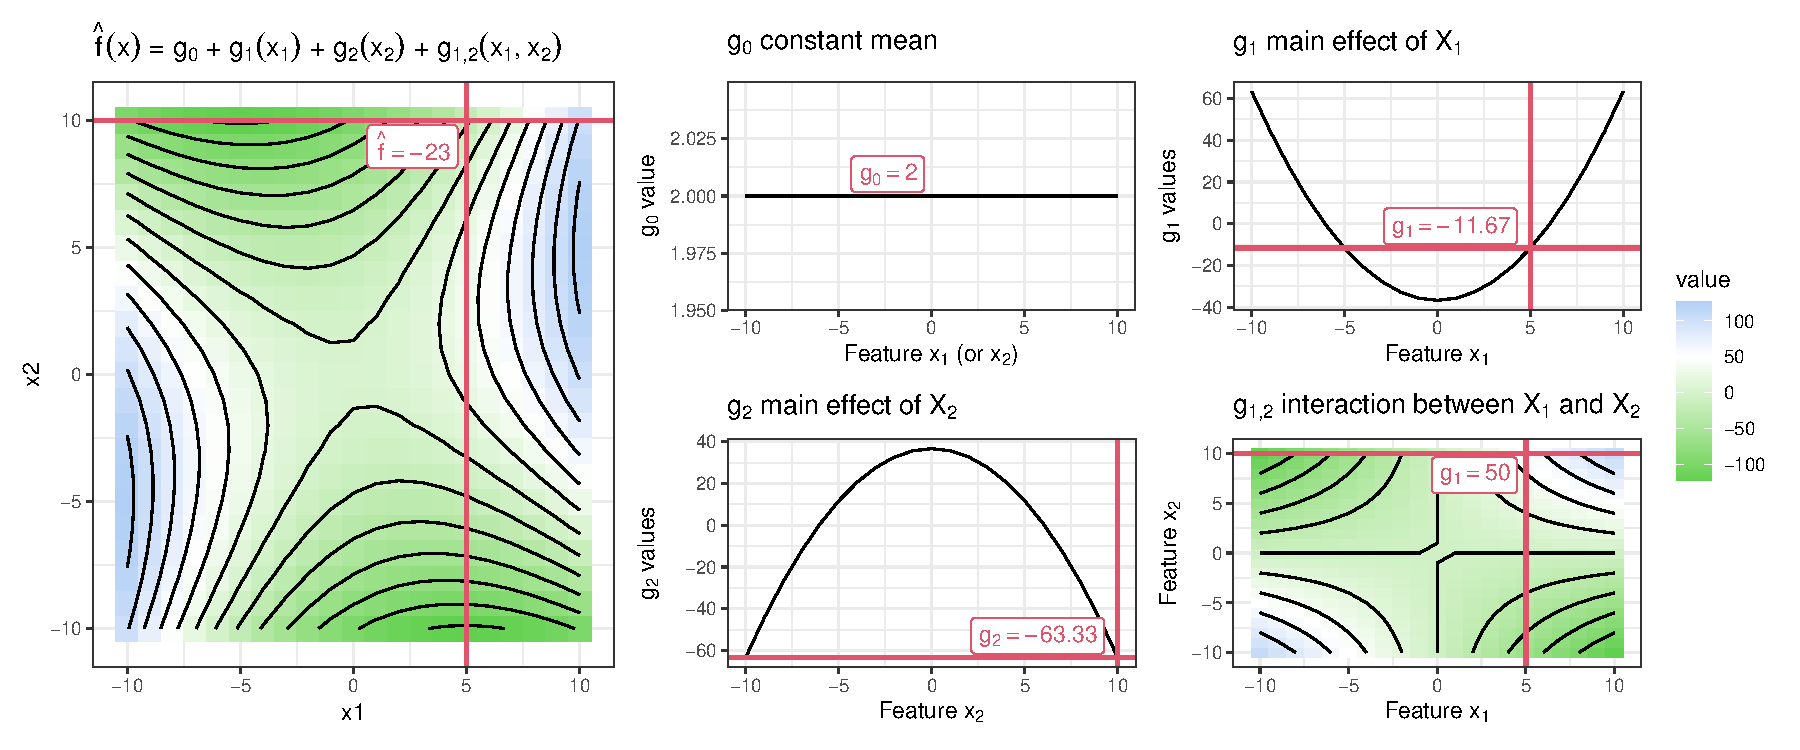
\includegraphics[width = \textwidth]{figure/decomposition}
        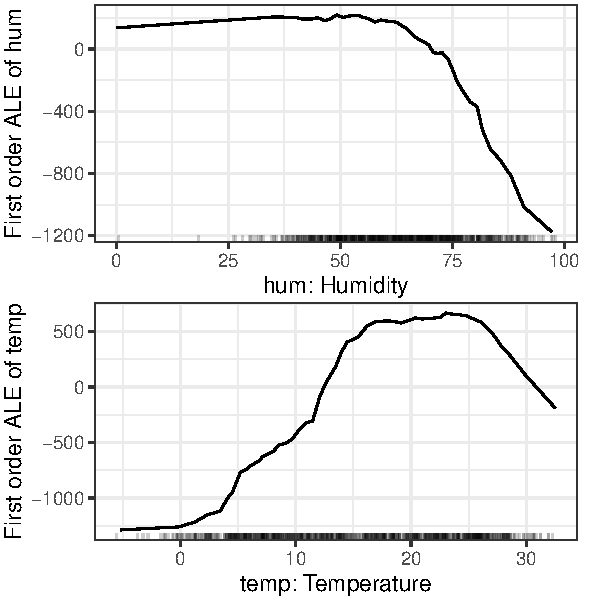
\includegraphics{figure/ale1d}
    \end{column}
    \begin{column}{0.5\textwidth}
        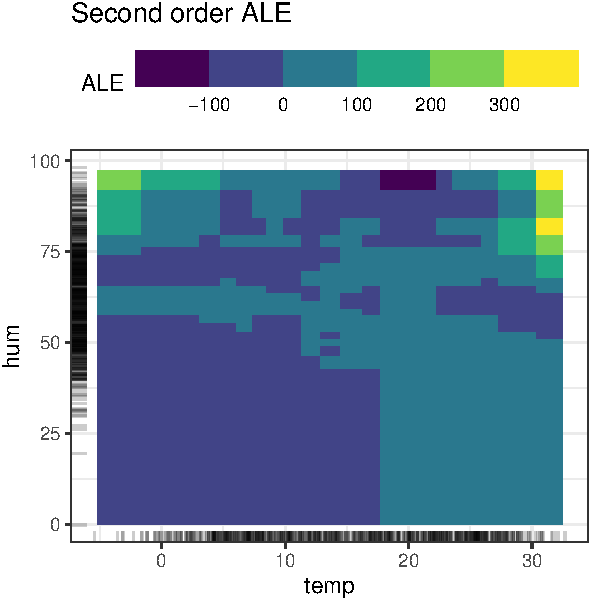
\includegraphics{figure/ale2d}
    \end{column}
    \end{columns}

    % \splitV{
        % \image{figure/ale1d}
    % }{
        % \image{figure/ale2d}
    % }
    
\end{frame}

\begin{frame}{ALE Decomposition}

    \begin{itemize}
        \item One can define ALE plots for arbitrary many variables \\
        (similar to PDPs vs. PD-functions)
        \item[$\rightarrow$] Gives full functional decomposition of ALE plots
        \pause
        \item \textbf{Advantages:} Handle dependencies well + computationally fast
        \item Constraints / orthogonality properties more complicated
        \item[$\implies$] ALE decomposition theoretically more involved, but good alternative in practice
    \end{itemize}
    
\end{frame}

% \begin{frame}{Sobol-Hoeffding decomposition}
    
% \end{frame}

% \begin{frame}{if enough time: Constraints (theory) for these other methods}

%     NB: Even more possible constraints (leading to ever more different decompositions) have been developed in research papers.
    
% \end{frame}

\begin{frame}{Conclusion: How useful are functional decompositions?}

    % Obwohl fDecompositions eigtl (aus Interpretability-Sicht) die Lösung für alles wären / theoretisch die Endlösung sind, sind alle anderen Methoden trotzdem nötig, weil fDecompositions sehr schwierig \& kompliziert zu berechnen sind
    % - Computation time skaliert exponentiell mit der Dimension / Anzahl features  =>  i.a. ist Erzwingen einer sparsen decomposition (s. GAMs / RPFs) die einzige realisitische Möglichkeit

    \begin{itemize}
        
        \item If computed, offer a lot of insight into a model or function, i.p. high-dimensional
        \item[$\rightarrow$] Complete analysis of all interactions
        \pause
        \item Very important theoretical concept:
        \begin{itemize}
            \item Theoretical framework for general definition of interactions (H-statistic)
            \item Theoretical background for many IML methods:
                GAMs and EBMs, 
                ICE, PDPs and PD-functions,
                ALE plots,
                Shapley values,
                Feature importance methods (see later)
            % \item GAMs and EBMs
            % \item ICE, PDPs and PD-functions
            % \item ALE plots
            % \item Shapley values (see later)
            % \item Feature importance methods (see later)
        \end{itemize}
        \pause
        \item In practice often infeasible ($2^p$ components for $p$ features)
        \item[$\implies$] Often only sparse decompositions feasible (E.g. EBMs)
        \pause
        \item All single methods have disadvantages:
        \begin{itemize}
            \item Standard fANOVA: Only independent features + compute intensive
            \item Generalized fANOVA: Even more computational intensive, evtl. infeasible
            \item ALE: No variance decomposition
        \end{itemize}
        
    \end{itemize}

    \pause
    % Nevertheless, functional decompositions are a very important concept in machine learning interpretability because they explain the idea behind many other methods and enable a much better understanding of other methods.
    \textbf{Overall:} Very important concept and theoretical background, explains idea behind many other methods
    
\end{frame}










\endlecture
\end{document}
